\documentclass[11pt]{article}
\usepackage[margin=1in]{geometry}
\usepackage{graphicx}
\usepackage{subcaption}
\usepackage{url}
\usepackage{dirtree}
\usepackage{hyperref}
\usepackage{longtable}
\usepackage{bbm}
\usepackage{amsfonts}
\usepackage{amsfonts}
\usepackage{xcolor}

\usepackage{glossaries}

\makeglossaries{}

\newglossaryentry{CI/CD}{
  name={CI/CD},
  description={Continuous Integration and Continuous Development. The process of
  automating software testing, building, and deployment.}
}

\newglossaryentry{CLI}
{
    name={CLI},
    description={A command-line interface (CLI) is a text-based user interface (UI) used to run programs, manage computer files and interact with the computer.}
}

\newglossaryentry{DSL}
{
    name=DSL,
    description={A computer language that is specialized to a particular application/domain}
}

\newglossaryentry{target execution}
{
    name=target execution,
    description={An instance of a \gls{target} that needs to be completed as per described in the project definition}
}

\newglossaryentry{cache}
{
    name=cache,
    description={to save something to computers memory or local storage. An example would be the output of a \gls{target execution}}
}

\newglossaryentry{project definition}
{
    name=project definition,
    description={A file containing information pertaining a project, an example could be the language that was used}
}

\newglossaryentry{metadata}
{
    name=metadata,
    description={any custom data that the project owner wants to add about the project}
}

\newglossaryentry{target}
{
    name=target,
    description={An execution target, a recipe or command for what you want to do to/with the project, ie build and deploy the project, run tests, ect}
}

\newglossaryentry{monorepo}
{
  name=monorepo,
  description={A software-development strategy in which the code for a number of projects is stored in the same repository.}
}

\title{\textbf{4ZP6 Capstone Project --- Prototype Document}}
\author{Usman Asad --- asadu  --- 400199934\\
  Ali Khan --- khana238  --- 400211680\\
  Omar Alkersh --- alkersho --- 400214491 \\
  Ahmed Al-sabounchi --- alsaboaa --- 001327403 \\
  Tanveer Shakeel --- shakeelt --- 400226915}

\begin{document}

\maketitle
\tableofcontents
\newpage

\section{Introduction}

\subsection{Purpose}

This document is intended to be read by programmers, it contains the projects design
decisions pertaining to the software architecture, language, application format,
and internal module API. The focus of the documentation is to provide guidance on the
processes of the program, an overview of how the program works, along with how the internal
code works and is structured. The document is meant to be a reference for the project, so if
any new developers want to contribute to the project, they can refer to this document to get
a better understanding of the project.

\subsection{Scope}

This project is a compiled \Gls{CLI} tool used to manage \glspl{monorepo}. This
tool should allow the user to check for changes in the code, execute \glspl{target},
check project dependencies, and provide tooling to aid in \Gls{CI/CD} pipelines
where appropriate. The project is built using the Go programming language.
\\\\
The goal is to provide a portable, fast, and easy to use program to help in
CI/CD pipelines for \glspl{monorepo}.

\subsection{Overview}
This document consists of information describing the entire architecture of the system, a programmatic
description of our implementation at the component/module level, and diagrams clarifying the design of
our product. Furthermore there will be a section thuroughly explaining how to use our tool. The current
product is just a prototype so the design is subject to change.
\\\\
The decision mainly consists of the language choice and the architecture. The
module design is meant to clarify the module breakdown, the API of each module,
and the module interactions and dependencies. The
\hyperref[sec:diagrams]{Diagrams} section provides more insight on the operation
of the program and how different modules interact with each other. The diagram
section is more concrete compared to the other sections and is not as likely
to change.
\\\\
For the module specifications, the sub items in the exported types represent
state variables.

\subsection{Definitions}

\printglossary[title=\normalsize\vspace*{-1.5\baselineskip}, toctitle=]

\section{Instructions}
The tool made here is a command line tool targeted at Unix Machines. It is written in Go, so you need to have Go installed on your machine to run the program. We are using golang version 1.19
\\\\
You can call \texttt{./cigo -h} to get the help output printed to the terminal.
\\\\
Feel free to add the program to your path.
\\\\
\textbf{Warning:} this program is targeted to Unix machines. Windows is not supported. If you are using Windows, you can use WSL to run the program.

\subsection{Sample Usage}
This repo is already setup with the files that we need to run the program. In the root directory, we have our \texttt{workspace.json}
file which contains information about our workspace. We also have sample projects in the \texttt{/apps} directory, each setup with their own \texttt{project.json} files.
\\\\
\textbf{Compiling the program:}
\\
First navigate to wherever the source code is located.
\\\\
\texttt{cd /src/}
\\\\
Use the command \textbf{go build} to generate the \textbf{cigo} binary. A new file should appear in your current directory.
\\\\
\texttt{go build}
\\\\
You can then use the compiled tool to manage your monorepo.
\\\\
\textbf{Creating schemas to test your workspace and project files against:}
\\
Let's create JSON schema's that help us validate our workspace and project files. To create these schemas we
call the \texttt{create-schema} command, passing it the type of schema we want to create (`workspace' or `project').
\\\\
\texttt{./cigo create-schema workspace}
\\\\
\texttt{./cigo list}
\\\\
You can search all the projects with key:value pairs by using the following command:
\\\\
\texttt{./cigo search name:proj\_a}
\\\\
We have a list command that lists all the projects in the workspace:
\\\\
\texttt{./cigo list}
\\\\
All other commands and functionality can be displayed through the use of the help function:
\\\\
\texttt{./cigo -h}
\\\\
Currently \texttt{run} \& \texttt{get-changed} are not implemented yet.

\section{System Overview}

The program is a \Gls{CLI} tool to manage \glspl{monorepo} and aid in
\gls{CI/CD} operations. It is meant to be light weight \& portable, and has no
trivial dependencies. The tool provides the abilities to run \glspl{target}
concurrently, define dependencies on the project level, and on the operation
level. It should also be able to perform operations on the projects; including
but not limited to creating, searching, and listing.
\\\\
A number of companies use the \gls{monorepo} development philosophy, and more
are adopting it. Without considering in-house solutions, there is currently only
one real competitor in this space with others catching up. \Glspl{monorepo} are
more complicated to manage than traditional repositories, greatly benefiting
from a tool to help automate and manage them.
\\\\
There other \gls{monorepo} tools in the space such
as; \href{https://nx.dev/}{NX}, \href{https://bazel.build/}{Bazel}, and others.
All of them have features that the others lack, or are slow to run or slow to
load in \gls{CI/CD} environments (NX is a node application).
\\\\
This program is aimed to combine their strengths, and best features based on our
experience with them. It is meant to fill a gap that none of these programs fill.

\section{System Architecture}
\label{sec:architecture}
\subsection{Architectural Design}

We have opted for a ``component'' based architecture. The different features and
logic are encapsulated in different components and modules as described in the
\hyperref[sec:modules]{Modules} section.
\\\\
%% Talk about the different modules and the functions that they need to fulfill
In the repository you will find a \texttt{/src} folder, which contains the source code for
the program. The entry point of the program is the \texttt{main.go} file. In the root of
the \texttt{/src} folder, you will also find the \texttt{go.mod} and \texttt{go.sum} files.
These files are used by the Go compiler to manage dependencies that are used throughout the program.
they are similar to the \texttt{package.json} \& \texttt{package-lock.json} files in a node application.
The source code is organized into different modules, modules are stored folders categorizing them under the \texttt{/src/pkg} folder
If a Module has a corresponding test file, it would be located in the same folder as the module. The test files are named after the
module they are testing, and are suffixed with \texttt{\_test.go}. When you want run the program you run the command
\texttt{go build} and it would compile a binary named \texttt{cigo} in the root of the \texttt{/src} folder. The
\texttt{cigo} binary is the executable that you can run to use the program.
\\\\
There are 6 modules; \texttt{commandParser}, \texttt{parser}, \texttt{data}, \texttt{algorithms}, \texttt{commands} and \texttt{misc}.
Each of the packages contain one or more \texttt{.go} file.
\begin{itemize}
\item \texttt{commandParser} package contains the \texttt{commandParser.go} module and is responsible for parsing the users input and
running the correct command. It also provides any specialized data definitions.

\item The \texttt{parser} package contains the /texttt{parser.go} module and provides functions to parse files to their
respective data types, (eg Parsing a workspace file to a workspace struct)

\item The \texttt{data} package contains the \texttt{data.go} module and provides the data definitions for the program. Mainly the
\gls{project definition} and workspace definitions.

\item The \texttt{alorithms} package contains the module /texttt{scheduler.go} which provides functions and data types to schedule the
execution of \gls{target} and tasks. This package also contains the \texttt{graph.go} module which provides functions and data types
to represent the dependency graphs of projects within the workspace.

\item The \texttt{commands} package contains the modules with the same name as the commands that the program supports. This package
has the \texttt{list.go}, \texttt{search.go}, and \texttt{schema.go} modules, each of which contains the logic for the corresponding
command. The \texttt{schema.go} module is responsible for generating the schema for the workspace file. The \texttt{list.go} module
is responsible for listing the projects in the workspace. The \texttt{search.go} module is responsible for searching for data within
projects in the workspace.

\item The \texttt{misc} package is a utility package that contains the \texttt{misc.go} module, it is mainly a workaround to Golang's import
limitation. It doesn't allow cyclic imports. This module should contain all
the common functionality to avoid cyclic imports.
\end{itemize}
Example module directory structure with a module named \texttt{data}:


\dirtree{%
  .1 src/.
  .2 \text{\color{magenta}cigo}.
  .2 main.go.
  .2 go.mod.
  .2 go.sum.
  .2 pkg/.
  .3 data/.
  .4 data.go.
  .4 data\_test.go.
  .3 \ldots{}.
}
\subsection{Design Rationale}
\subsubsection{Language}
\label{sec:lang}

The language that we decided to write the program in is Go. We needed a compiled
and type checked language. We decided to choose Go over C/C++ and Java due to usability and
safety concerns. C/C++ have the memory issues that needs to be addressed and managed; and
Java is disliked and slow. Furthermore, it requires a JVM to be installed, which
defeats the purpose of small installation size.
\\\\
We also considered Rust, but decided against it due to the learning curve and
the majority of the team not having experience with it.

\subsubsection{Software Architecture}

We decided on a component based design. This should allow us to expand the
software without significant rewrites when we want to extend its functionality.
In addition, it allows us to work on separate parts in parallel accelerating
development.
\\\\
Most other software architectures, client-server or MVC, are not relevant to
this project nor do they provide any benefit. This program consists only of a
compiled CLI program, no external communication is required in this iteration.

\subsection{File System}
The monorepo tool being developed uses the file system to store data that is used throughout the project. We need to maintain
a certain structure in the file system, files are constantly being read and we need to make sure that the files are in the correct structure.
\\
The file system structure is as follows:
\begin{itemize}
  \item There must be a workspace file named \texttt{workspace.json} in the root of the repository/monorepo.
  This file contains information regarding the workspace, such as the name of the workspace, projects in the
  workspace, project paths, etc.
  \item Every project path listed in the workspace file must be a valid path to a project. A project is a folder that contains a
  project file named \texttt{project.json}. This file contains information regarding the project, such as the \glspl{target} to
  be executed, project dependencies, etc.
\end{itemize}
More information regarding the structure of the \texttt{workspace} and \texttt{project definition} files can be found in the \hyperref[mod:data]{Data} module subsection.
\subsection{Decomposition}

The following diagram mainly concerns itself with the ``import'' relation that
the components have, which component imports which component. There is no
inheritance or extension relation. All the data types are defined once and not
extended beyond their definition.

\subsubsection{Diagrams}

\begin{figure}[h!]
  \centering
  \begin{subfigure}{0.5\linewidth}
    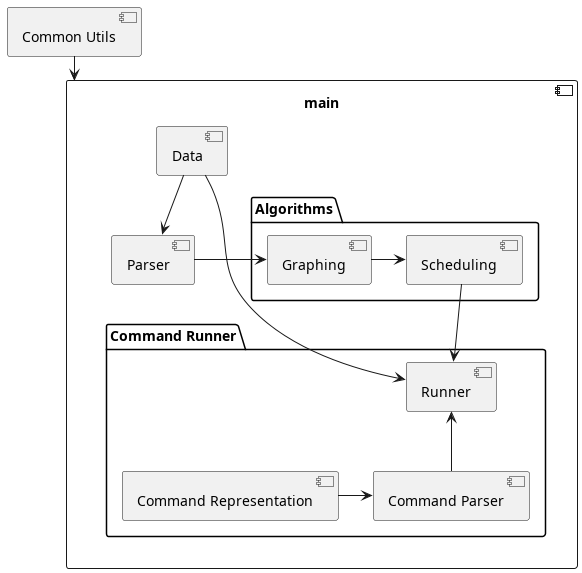
\includegraphics[width=\linewidth]{diags/components.png}
    \caption{\label{fig:comp}Component Diagram}
  \end{subfigure}
  \begin{subfigure}{0.15\linewidth}
    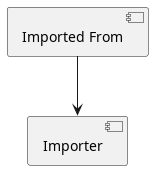
\includegraphics[width=\linewidth]{diags/comp_legend.png}
    \caption{\label{fig:comp}Legend}
  \end{subfigure}
  \caption{Component Composition Diagram}
\end{figure}
\newpage

\begin{figure}[h!]
\end{figure}

\begin{figure}[h!]
  \centering
  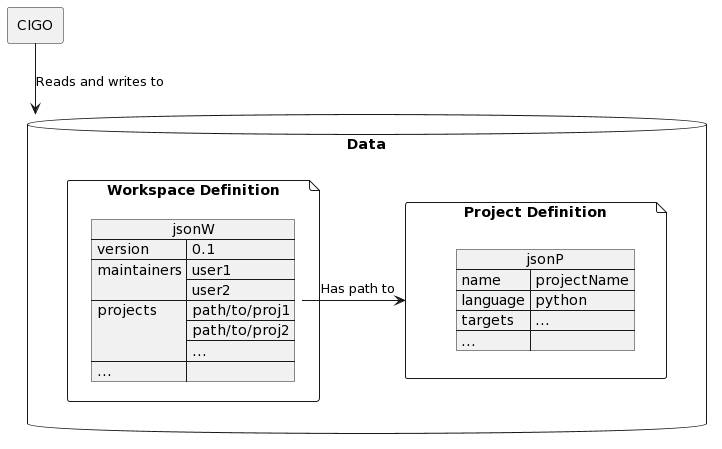
\includegraphics[width=0.8\linewidth]{diags/system.png}
  \caption{Data Interaction and store}
  \label{fig:storage}
\end{figure}

Note that the data can be stored as a JSON, YAML, or a DSL that is yet to be
developed. See figure \ref{fig:storage}.


\newpage
\section{Modules}
\label{sec:modules}

One module may export multiple types and
define functions over many types. No function is assumed to be a ``class method''
unless specified. We are following go langs package convention where each folder under the \texttt{/src/pkg/} folder is a package/module
and all the \texttt{*.go} files in that package are part of that module.

\subsection{Module: `commandParser'}
\label{mod:command}

\subsubsection{Exported Types}

The exported types are representations of the possible command line arguments
that the program accepts. They are used to parse them and represent them in
code. The sub items are struct fields, which represent options or the command.

\begin{itemize}
\item $Args$:
  \begin{itemize}
  \item help: $Boolean$
  \item dry run: $Boolean$
  \item version: $Boolean$
  \item command: $Command$
  \end{itemize}
\item $Command$ --- enum:
  \begin{itemize}
  \item $List$
  \item $Search$:
    \begin{itemize}
    \item searchItems: $map[key]value$

    \item limit: $\mathbbm{N}$
    \end{itemize}
  \item $Run$:
    \begin{itemize}
    \item project: $string | seq(string)$
    \item target: $string$
    \end{itemize}
  \item $GetChanges$:
    \begin{itemize}
    \item baseRef: $string$
    \item targetRef: $string | null$
    \end{itemize}
  \item $CreateSchema$:
    \begin{itemize}
      \item type: $string$
    \end{itemize}
  \end{itemize}
\end{itemize}

\subsubsection{Functions}

\begin{tabular}[h!]{l|l|l|p{6cm}}
  \textbf{Name} & \textbf{Input} & \textbf{Output} & \textbf{Description} \\
  \hline
  Parse & string & Args & Parses the command arguments to an $Args$ type.\\
  \hline
  Run & Args & $\mathbbm{Z}$ & Runs the given command based on the data within. Returns the command success code.\\
  \hline
  GetCommand & & Command & Returns the command that is to be executed.\\
\end{tabular}

\vspace{2em}

\textbf{Definitions}\\

$Parse(string):$
\begin{itemize}
\item transition:
  \begin{itemize}
  \item $help :=$ The help flag is present.
  \item $dryRun :=$ The dry run flag is present.
  \item $version :=$ The version flag is present.

  \item $command :=$ The sub command to execute.
  \end{itemize}
\item output: $out := Self$
\item exception: $exc :=$ Parse failure.
\end{itemize}

\vspace{1em}

$Run(args):$
\begin{itemize}
\item output: $out :=$ The command status code. Non-zero if the command failed.
\item exceptions: None
\end{itemize}
\vspace{1em}

$GetCommand():$
\begin{itemize}
\item output: $out :=$ The command that is to be executed
\item exceptions: None
\end{itemize}

\subsection{Module: `parser'}
\label{mod:parser}
This module contains code for reading project definitions and workspace/repo files
in .yaml, .json or from our Domain Specific Language
\subsubsection{Uses/Imports}
\begin{itemize}
  \item Data Module
  \item External JSON library
  \item External YAML library
\end{itemize}

\subsubsection{Exported Types}
\begin{itemize}
  \item Parser = ?
  \item FileType = {JSON, YAML, DSL}
\end{itemize}

\subsubsection{Functions}
\begin{longtable}{l|l|l|l}
  \textbf{Name} & \textbf{Inputs} & \textbf{Output} & \textbf{Description} \\ \hline
  DecodeProjectDef &
    String, FileType &
    ProjectDefinition &
    \begin{tabular}[c]{@{}l@{}}Takes in a filePath, and a file type,\\decodes the file and returns an\\instance of a ProjectDefinition struct\end{tabular} \\\hline
  EncodeProjectDef &
  \begin{tabular}[c]{@{}l@{}}ProjectDefinition, \\ string, \\ FileType\end{tabular} &
    Encoded String &
    \begin{tabular}[c]{@{}l@{}}Takes in a ProjectDefinition, a file path,\\and a FileType and writes\\the deserialized content to the file.\end{tabular} \\\hline
  DecodeWorkspace &
    String, FileType &
    Workspace &
    \begin{tabular}[c]{@{}l@{}}Takes in a filePath, and a file type,\\decodes the file and returns an\\instance of a Workspace struct\end{tabular} \\\hline
  EncodeWorkspace &
    \begin{tabular}[c]{@{}l@{}}Workspace, \\String, \\ FileType\end{tabular} &
    Encoded String &
    \begin{tabular}[c]{@{}l@{}}Takes in a Workspace, a file path,\\and a FileType and writes the\\deserialized content to the file.\end{tabular}
  \end{longtable}

  \vspace{2em}
  \textbf{Definitions}\\

  $DecodeProjectDef(filePath, fileType):$
  \begin{itemize}
  \item output: $out :=$ The serialized ProjectDefinition.
  \item exception: $exc :=$
    \begin{align*}
      \text{ file doesn't exist } &\implies FileNotFound|\\
      \text{ serialization error } &\implies InvalidFormat|\\
      True &\implies none
    \end{align*}
  \end{itemize}

  \vspace{1em}
  $EncodeProjectDef(projDef, filePath, fileType):$
  \begin{itemize}
  \item output: $out :=$ Write to the file the deserialized project definition.
  \item exception: $exc :=$
    \begin{align*}
      \text{ Failed to write } &\implies IOError|\\
      \text{ Bad path } &\implies IllegalPath|\\
      \text{ deserialization error } &\implies EncodingErr|\\
      True &\implies none
    \end{align*}
  \end{itemize}

  \vspace{1em}
  $DecodeWorkspace(filePath, fileType):$
  \begin{itemize}
  \item output: $out :=$ The serialized Workspace.
  \item exception: $exc :=$
    \begin{align*}
      \text{ file doesn't exist } &\implies FileNotFound|\\
      \text{ serialization error } &\implies InvalidFormat|\\
      True &\implies none
    \end{align*}
  \end{itemize}

  \vspace{1em}
  $EncodeWorkspace(workspace, filePath, fileType):$
  \begin{itemize}
  \item output: $out :=$ Write to the file the deserialized workspace definition.
  \item exception: $exc :=$
    \begin{align*}
      \text{ Failed to write } &\implies IOError|\\
      \text{ Bad path } &\implies IllegalPath|\\
      \text{ deserialization error } &\implies EncodingErr|\\
      True &\implies none
    \end{align*}
  \end{itemize}

\subsection{Module: `algorithms'}
\label{mod:algorithms}
\subsubsection{Exported Types}
\begin{itemize}
\item ISchedule = ?
\item IGraph = ?
\end{itemize}

\subsubsection{Functions}
\begin{tabular}{l | l | l | p{7cm} }
  \textbf{Name} & \textbf{Input} & \textbf{Output} & \textbf{Description} \\
  \hline
  ScheduleJobs & Graph & sec(string) & Returns a scheduling for the job execution based on the given graph \\
  \hline
  GraphProjects & sec(Project) & Graph & Uses Project to see dependant file(s) and links together as tree, returns
                                         a dependency graph. \\
  \hline
  projectHash & Project & string & Returns a hash of the project. (currently the project name) \\
\end{tabular}

\vspace{2em}
\textbf{Definitions}\\

$ScheduleJobs(graph):$
\begin{itemize}
\item output: $out :=$ A parallelized schedule to execute jobs while
  respecting dependencies.
\item exception: $exc :=$ None.
\end{itemize}

\vspace{1em}
$GraphProjects(graph):$
\begin{itemize}
\item output: $out :=$ The projects dependency graph
\item exception: $exc :=$ CyclicDependency.
\end{itemize}

$projectHash(ProjectDefinition):$
\begin{itemize}
\item output: $out :=$ The projects name
\item exception: $exc :=$ None
\end{itemize}

\subsection{Module: `data'}
\label{mod:data}
The following modules represent the objects that are used as templates for storing the Project Definition, Workspace, and Target information accordingly. They are all part of the same package.

\begin{enumerate}
\item ProjectDefinition
\item Workspace
\item Target
\end{enumerate}

\subsubsection{Exported Types}
\begin{itemize}
\item ProjectDefinition = ?
\item ProjectDefintionBuilder = ?
\item Workspace = ?
\item WorkspaceBuilder = ?
\item Target = ?
\item TargetBuilder = ?
\end{itemize}

\subsubsection{Non-Exported Types}
\begin{itemize}
\item DependsTarget = ?
\end{itemize}

\newpage
\subsubsection{Types Members}

Tables showing the data type members. All are assumed to be public as they are
used to created and validate the definition files. Note that the exact names are
subject to change.

\begin{table}[h!]
  \centering
  \begin{tabular}[h!]{l | l | c | l}
    \textbf{Name} & \textbf{Type} & \textbf{Required} & \textbf{Description}\\
    \hline
    MainLanguage & string & True & The main language of the project\\
    \hline
    LangVersion & string & False & The language version or standard\\
    \hline
    Name & string & True & The project name\\
    \hline
    Targets & map[string]Target & True & The list of \glspl{target}. The key is
                                         the target name\\
    \hline
    Version & string & False & Project version\\
    \hline
    Owners & seq(string) & True & The list of project owners/maintainers\\
    \hline
    DependsOn & seq(string) & True & The list of project it depends on\\
    \hline
    Metadata & map[string]string & False & Custom metadata\\
    \hline
    AffectsTags & seq(string) & True & Tags that this project affects\\
    \hline
    AffectedByTags & seq(string) & True & Tags that this project is affected by
  \end{tabular}
  \caption{The ProjectDefinition}
  \label{table:proj_def}
\end{table}

\begin{table}[h!]
  \centering
  \begin{tabular}[h!]{l | p{3cm} | c | p{7cm}}
    \textbf{Name} & \textbf{Type} & \textbf{Required} & \textbf{Description}\\
    \hline
    Project & string & True & Project Name\\
    \hline
    Target & string & True & Target Name\\
  \end{tabular}
  \caption{The DependsTarget}
  \label{table:dependstARGET}
\end{table}

\begin{table}[h!]
  \centering
  \begin{tabular}[h!]{l | p{3.5cm} | c | p{7cm}}
    \textbf{Name} & \textbf{Type} & \textbf{Required} & \textbf{Description}\\
    \hline
    DependsOn & seq(DependsTarget) & True & Target dependencies\\
    \hline
    Cmds & seq(string) & True & The commands to run for this target\\
    \hline
    Artifacts & seq(string) & True & The paths to the generated artifacts, could
                                     be a directory.\\
    \hline
    Env & map[string]string | seq(string) & True & Environment variables
  \end{tabular}
  \caption{The Target}
  \label{table:target}
\end{table}

\begin{table}[h!]
  \centering
  \begin{tabular}[h!]{l | l | c | l}
    \textbf{Name} & \textbf{Type} & \textbf{Required} & \textbf{Description}\\
    \hline
    Owners & seq(string) & True & The list of repo maintainers.\\
    \hline
    AppVer & string & True & The program version this file is compatible with.\\
    \hline
    Projects & map[string]string & True & List of paths to project files.\\
    \hline
    Tags & seq(string) & True & List of available tabs.\\
    \hline
    RequiredTargets & seq(string) & True & Required list of targets to be
                                           defined.\\
    \hline
    RemoteUrl & string & False & Where is this repo hosted.
  \end{tabular}
  \caption{The Workspace}
  \label{table:workspace}
\end{table}

\begin{table}[h!]
  \centering
  \begin{tabular}[h!]{l | l | c | l}
    \textbf{Name} & \textbf{Type} & \textbf{Required} & \textbf{Description}\\
    \hline
    projectDefinition & ProjectDefinition & True & The ProjectDefinition to be built.\\
  \end{tabular}
  \caption{The ProjectDefinitionBuilder}
  \label{table:projectDefBuilder}
\end{table}

\begin{table}[h!]
  \centering
  \begin{tabular}[h!]{l | l | c | l}
    \textbf{Name} & \textbf{Type} & \textbf{Required} & \textbf{Description}\\
    \hline
    workspace & Workspace & True & The Workspace to be built.\\
  \end{tabular}
  \caption{The WorkspaceBuilder}
  \label{table:WorkspaceBuilder}
\end{table}

\begin{table}[h!]
  \centering
  \begin{tabular}[h!]{l | l | c | l}
    \textbf{Name} & \textbf{Type} & \textbf{Required} & \textbf{Description}\\
    \hline
    target & Target & True & The Target to be built.\\
  \end{tabular}
  \caption{The TargetBuilder}
  \label{table:targetBuilder}
\end{table}


\subsubsection{Functions}
We are utilizing a
\href{https://en.wikipedia.org/wiki/Builder\_pattern}{builder pattern} to
create the objects. Each of the types has its own `setter'
functions for its fields as well. The setter functions and the builder functions are omitted from the documentation
due to their number and simplicity.\\\\
The only thing to note is that each of the builder types has a \texttt{Build()} function which returns the constructed
object.

\subsection{Module: `commands'}
\label{mod:commands}
This module contains the logic for all the different commands that are available in the program. Each command has its own
file in the \texttt{commands} directory
\subsubsection{Exported Types}
\begin{itemize}
\item N/A
\end{itemize}

\subsubsection{Types}
\begin{itemize}
\item search = ?
\end{itemize}

\subsubsection{Types Members}

Tables showing the data type members.

\begin{table}[h!]
  \centering
  \begin{tabular}[h!]{l | l | c | l}
    \textbf{Name} & \textbf{Type} & \textbf{Required} & \textbf{Description}\\
    \hline
    Name & string & True & The project name\\
    \hline
    MainLanguage & string & True & The main language of the project\\
    \hline
    Targets & map[string]Target & True & The list of \glspl{target}. The key is
                                         the target name\\
    \hline
    Version & string & False & Project version\\
    \hline
    Owners & seq(string) & True & The list of project owners/maintainers\\
    \hline
    DependsOn & seq(string) & True & The list of project it depends on\\
    \hline
    AffectsTags & seq(string) & True & Tags that this project affects\\
    \hline
    AffectedByTags & seq(string) & True & Tags that this project is affected by\\
    \hline
    Others & map[string]string & False & Custom metadata\\
  \end{tabular}
  \caption{The search type}
  \label{table:search}
\end{table}

\subsubsection{Functions}
\begin{tabular}{l | l | l | p{7cm} }
  \textbf{Name} & \textbf{Input} & \textbf{Output} & \textbf{Description} \\
  \hline
  List &  &  & Prints all the projects in the workspace onto the console \\
  \hline
  CreateSchema & string & File & Generates a schema for the corresponding type (Workspace or ProjectDefinition)\\
  \hline
  mapToSearch & map[string]string & search & Given a map of search parameters, it returns a search object.\\
  \hline
  contains & seq(string), string & bool & Given a list of strings and a string, it returns true if the string is in the list.\\
  \hline
  Search & map[string]string & seq(ProjectDefinition) & Given a map of search parameters, it returns a list of projects that match the search parameters.\\
\end{tabular}

\vspace{2em}
\textbf{Definitions}\\

$List():$
\begin{itemize}
\item output: $out :=$ None.
\item exception: $exc :=$ None.
\end{itemize}

\vspace{1em}
$CreateSchema(type):$
\begin{itemize}
\item output: $out :=$ schema json file
\item exception: $exc :=$ IOError
\end{itemize}

$mapToSearch(searchQueries):$
\begin{itemize}
\item output: $out :=$ search object
\item exception: $exc :=$ None
\end{itemize}

$contains(stringList, query):$
\begin{itemize}
\item output: $out :=$ true or false depending on if query is in stringList
\item exception: $exc :=$ None
\end{itemize}

$Search(searchQueries):$
\begin{itemize}
\item output: $out :=$ list of projects that match the search queries
\item exception: $exc :=$ IOError
\end{itemize}

\subsection{Module: `misc'}
\label{mod:misc}
This module contains miscellaneous functions that are used by other modules. It helps to avoid cyclic dependencies between modules.

\subsubsection{Exported Types}
\begin{itemize}
\item N/A
\end{itemize}
\subsubsection{Functions}
\begin{tabular}{l | l | l | p{7cm} }
  \textbf{Name} & \textbf{Input} & \textbf{Output} & \textbf{Description} \\
  \hline
  GetRoot &  & string & returns the root path of the monorepo\\
  \hline
  GetWorkspacePath &  & string & returns the path to the workspace file\\
  \hline
  GetRelativePath & string & string & returns the relative path of the given path\\
\end{tabular}

\vspace{2em}
\textbf{Definitions}\\

$GetRoot():$
\begin{itemize}
\item output: $out :=$ the root path of the monorepo as a string
\item exception: $exc :=$ IOError
\end{itemize}

$GetWorkspacePath():$
\begin{itemize}
\item output: $out :=$ the path to the workspace file as a string
\item  exception: $exc :=$ IOError
\end{itemize}

$GetRelativePath(path):$
\begin{itemize}
\item output: $out :=$ the relative path of the given path as a string
\item exception: $exc :=$ IOError
\end{itemize}


\newpage
\section{Diagrams}
\label{sec:diagrams}

\subsection{State Diagram}
Describes the possible states of the program

\begin{figure}[htbp]
  \centering
  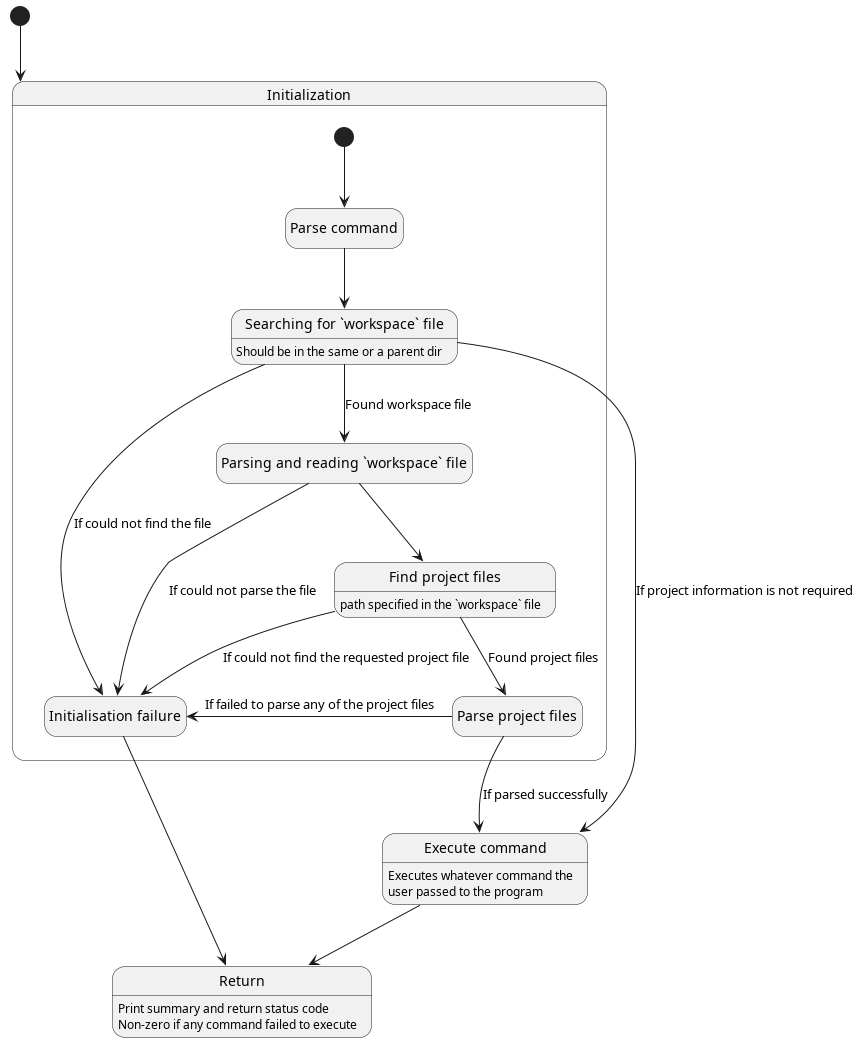
\includegraphics[width=0.5\textheight]{diags/state.png}
  \caption{\label{fig:state}State diagram}
\end{figure}

\newpage
\subsection{Activity Diagram}

Note that the activity diagram are broken into pieces for readability on PDF.
You can follow the figure order.

\subsubsection{Get Affected projects}

Describes how the program gets a list of affected projects.

\begin{figure}[htbp]
  \centering
  \begin{subfigure}{0.35\linewidth}
    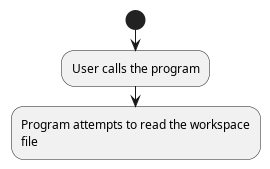
\includegraphics[width=\linewidth]{diags/get_affected_activity.png}
    \caption{Initialize}
  \end{subfigure}
  \begin{subfigure}{0.45\linewidth}
    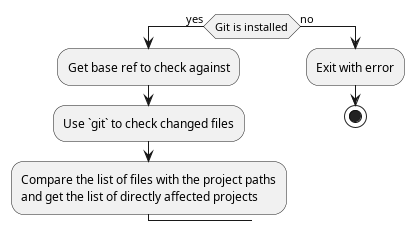
\includegraphics[width=\linewidth]{diags/get_affected_activity_001.png}
    \caption{Check Changes}
  \end{subfigure}
  \begin{subfigure}{0.5\linewidth}
    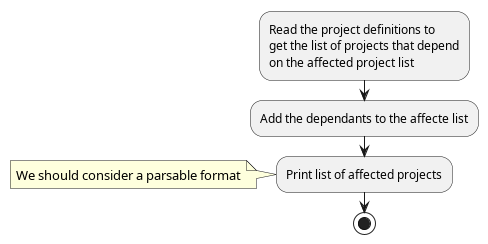
\includegraphics[width=\linewidth]{diags/get_affected_activity_002.png}
    \caption{Check Dependencies}
  \end{subfigure}
  \caption{\label{fig:act_aff}Get a List of Affected Projects}
\end{figure}

\subsubsection{Execute targets}

Shows the activity of the program when executing projects \gls{target}.

\begin{figure}[htbp]

  \begin{minipage}{0.45\textwidth}
    \centering
    \begin{subfigure}[b]{\linewidth}
      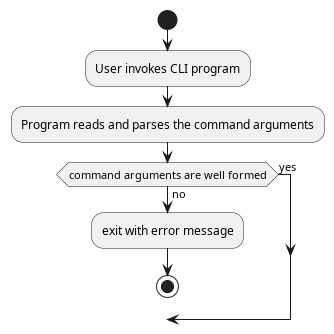
\includegraphics[width=\linewidth]{diags/activity.png}
      \caption{Get user input}
    \end{subfigure}

    \bigskip
    \addtocounter{subfigure}{1}

    \begin{subfigure}[b]{\linewidth}
      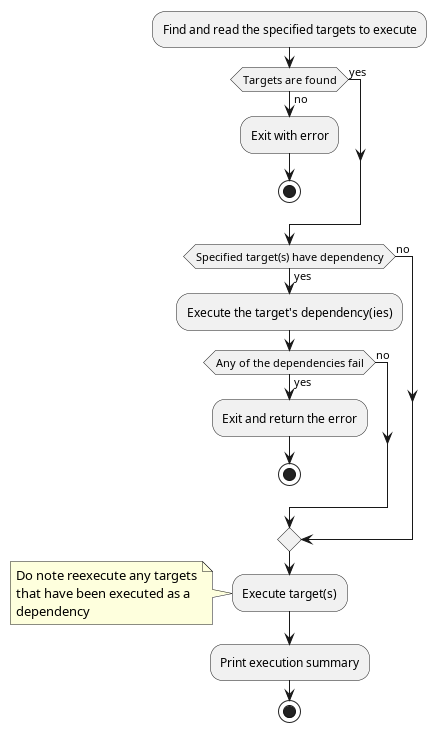
\includegraphics[width=\linewidth]{diags/activity_002.png}
      \caption{Execute}
    \end{subfigure}
  \end{minipage}
  \hfill
  \begin{minipage}{0.5\textwidth}
    \addtocounter{subfigure}{-2}
    \begin{subfigure}[b]{\linewidth}
      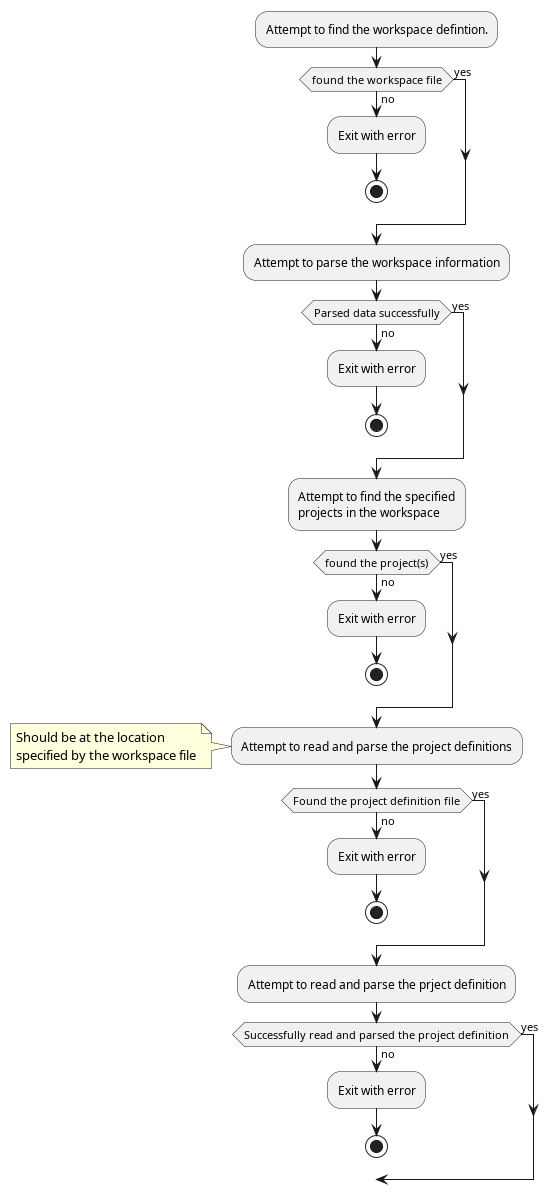
\includegraphics[width=\linewidth]{diags/activity_001.png}
      \caption{Initialize}
    \end{subfigure}
  \end{minipage}

  \caption{\label{fig:act_exec}Execute Project Targets}
\end{figure}

\clearpage

\subsubsection{Add Project}

\begin{figure}[h!]
  \centering
  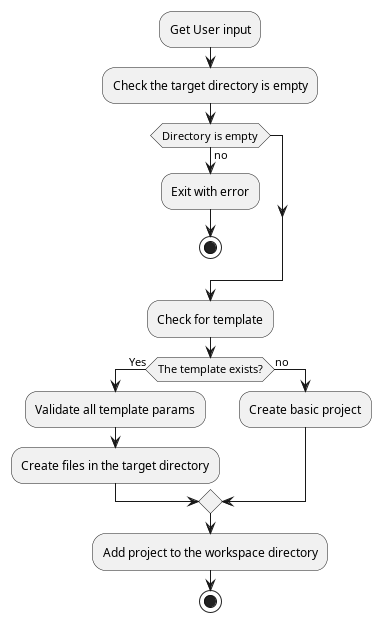
\includegraphics[height=0.6\textheight]{diags/add_proj.png}
  \caption{Add a new project}
  \label{fig:new_proj}
\end{figure}

\newpage
\subsection{Sample Repository Structure}

Sample project directory structure:

\dirtree{%
  .1 repo/.
  .2 .git/.
  .2 workspace\_def
  \ldots{}
  \begin{minipage}[t]{7cm}
    This file contains information about the entire
    repository{.}
  \end{minipage}.
  .2 path/to/.
  .3 proj1/.
  .4 src/...
  .4 proj\_def
  \ldots{}
  \begin{minipage}[t]{7cm}
    This file contains the project definition as described by
    the some previous section{.} All targets are executed from
    this location{.}
  \end{minipage}.
  .3 proj2/.
  .4 src\_file.
  .4 proj\_def.
}

\section{Requirements Traceability Matrix}

\begin{tabular}[h!]{c|p{5cm}|p{2cm}| p{4cm}}
  \textbf{Requirement} & \textbf{Description} & \textbf{Figure or section} & \textbf{Comments} \\
  \hline
  1 & Compiled & \ref{sec:lang} & Language choice \\
  \hline
  2 & \Gls{CLI} & \ref{mod:command} & \\
  \hline
  3 & Add Projects & \ref{mod:command}, \ref{fig:new_proj} & \\
  \hline
  4 & Language agnostic & \ref{fig:new_proj}, \ref{table:proj_def} & No design choice assumes the project language. The referenced diagram allows the user to specify the project template to be created.\\
  \hline
  5 & Define Target & \ref{mod:data}, \ref{fig:storage}, \ref{table:proj_def}, \ref{table:target} & Allows the user to define them to whatever they like. \\
  \hline
  6 & Define dependencies & \ref{fig:storage}, \ref{table:proj_def},
                            \ref{table:target} & \\
  \hline
  7 & Detect changes in dependencies & \ref{mod:command} & Defines the command to do so \\
  \hline
  8 & Produce dependency graph & \ref{mod:alg}, \ref{table:proj_def} & \\
  \hline
  9 & Define project dependency & \ref{fig:storage}, \ref{table:proj_def} & \\
  \hline
  10 & Dependency is respected & \ref{mod:alg}, \ref{table:proj_def} & \\
  \hline
  11 & List projects & \ref{mod:command}, \ref{table:workspace}& \\
  \hline
  12 & Return status of execution  & \ref{mod:command} & Returns the return code \\
  \hline
  13 & Preserve colored output & NA & This is highly dependent on the implementation \\
  \hline
  14 & Read project definition & \ref{mod:parser}, \ref{table:proj_def} & \\
  \hline
  15 & Detect malformed project definitions & \ref{mod:parser} & Returns an exception \\
  \hline
  16 & Project definition information & \ref{table:proj_def} & \\
  \hline
  17 & Define custom execution target & \ref{table:target}, \ref{table:proj_def} & \\
  \hline
  18 & Execute defined \glspl{target} & \ref{mod:command}, \ref{fig:act_exec}, \ref{table:target} & \\
  \hline
  19 & Define output artifact & \ref{table:target} & \\
  \hline
  20 & Print target output in realtime & NA & Depends on the implementation \\
  \hline
  21 & Execute targets concurrently & \ref{mod:alg} & Provides an execution schedule \\
  \hline
  22 & Target should fail if its dependencies fail & \ref{mod:alg}, \ref{table:target} & We can get the dependencies from the execution plan. Also dependent on the implementation\\
  \hline
  23 & Cache target execution & \ref{table:target} & Dependent on the implementation. \\
  \hline
  24 & Workspace file & \ref{mod:data}, \ref{fig:storage} &
\end{tabular}

\end{document}
